% =====================================================================
%  PROJECT REPORT — single column, report class, chapter structure
%  Long-Range Secure Messaging System Using ESP32 and LoRa
%
%  Build:  pdflatex project_report && bibtex project_report
%          && pdflatex project_report && pdflatex project_report
%
%  CHAPTER 7 (RESULTS) IS DELIBERATELY EMPTY. Hardware trials have not
%  been run. Fill it only with measurements you took yourself, and label
%  simulation as simulation.
%
%  CHECK BEFORE SUBMITTING: author names, USNs, guide name and
%  designation, academic year, and the department/college formatting your
%  institution requires on the title page.
% =====================================================================
\documentclass[12pt,a4paper,oneside]{report}

\usepackage[margin=1in,bindingoffset=0.35in]{geometry}
\usepackage{setspace}
\usepackage{times}
\usepackage{graphicx}
\usepackage{amsmath,amssymb}
\usepackage{booktabs}
\usepackage{array}
\usepackage{longtable}
\usepackage{url}
\usepackage{tikz}
\usetikzlibrary{shapes.geometric, arrows.meta, positioning, calc, fit, backgrounds}
\usepackage[hidelinks]{hyperref}

\onehalfspacing
\setlength{\parskip}{6pt}

\begin{document}

% =====================================================================
%  TITLE PAGE
% =====================================================================
\begin{titlepage}
\centering
\vspace*{0.5cm}

{\large B.M.S. COLLEGE OF ENGINEERING, BENGALURU}\\[0.2cm]
{\normalsize (Autonomous Institution affiliated to VTU)}\\[1.2cm]

{\large Department of Information Science and Engineering}\\[2.0cm]

{\large PROJECT REPORT}\\[0.6cm]

{\LARGE\bfseries Long-Range Secure Messaging System\\[0.3cm]
Using ESP32 and LoRa}\\[2.0cm]

{\normalsize Submitted in partial fulfilment of the requirements for the degree of}\\[0.3cm]
{\large\bfseries Bachelor of Engineering}\\[0.2cm]
{\normalsize in Information Science and Engineering}\\[1.8cm]

{\normalsize Submitted by}\\[0.4cm]
\begin{tabular}{ll}
R.~Rakshith      & \textit{[USN]} \\
S.~P.~Hegde      & \textit{[USN]} \\
S.~G.~Uppalli    & \textit{[USN]} \\
K.~S.~Suchit     & \textit{[USN]} \\
\end{tabular}\\[1.8cm]

{\normalsize Under the guidance of}\\[0.3cm]
{\large \textit{[Guide name]}}\\
{\normalsize \textit{[Designation], Department of Information Science and Engineering}}\\[1.5cm]

{\normalsize \textit{[Academic Year]}}

\end{titlepage}

% =====================================================================
%  ABSTRACT
% =====================================================================
\chapter*{Abstract}
\addcontentsline{toc}{chapter}{Abstract}

Radio that reaches a few kilometres is most useful where there is no
infrastructure, and yet the protocol usually built on LoRa, namely LoRaWAN,
assumes a gateway with a working internet connection behind it. Take the gateway
away and the network stops. This project builds a messaging system that does not
have that dependency.

Five nodes, each an ESP32-S3 paired with an SX1262 radio, form a mesh in which
every device sends, relays and receives. There is no central node and no
coordinator. A phone connects to any device over Bluetooth Low Energy and acts as
the keyboard and screen, while the node's own display carries local
diagnostics. Routing uses a
destination-sequenced distance-vector protocol whose updates travel inside the
neighbour-discovery beacon, so routing costs the network no transmissions of its
own; the beacon interval widens as a node learns of more nodes, which keeps
control traffic from growing with the mesh.

Messages are encrypted with AES-128-GCM under a key that two nodes agree between
themselves using X25519, mixed with a network key shared by all five. A relay
holds the network key and still cannot read what it forwards. The design that
makes this work across several hops is a packet whose endpoint addresses are
sealed by the cipher while the hop addresses, which relays have to rewrite, sit
outside the seal. On top of this the system adds link-layer frame authentication,
replay rejection that tolerates out-of-order arrival, delivery receipts the
destination proves cryptographically, and an outbox that holds a message for a
node that is temporarily unreachable instead of dropping it.

The firmware builds and passes a suite of host-side adversarial tests, and the
protocol has been exercised in a simulator at scales larger than the hardware we
have. Field trials on real radios have not been carried out. Chapter~7 is
therefore reserved for measured results and the method for obtaining them is set
out in Chapter~6.

\tableofcontents
\listoffigures
\listoftables

% =====================================================================
\chapter{Introduction}
% =====================================================================

\section{Background}

Mobile networks cover most of India most of the time, and that is exactly why
their absence is a problem when it happens. A cell tower needs power, a backhaul
link and a site that has not been flooded or shaken. Disasters remove all three
at once, and they remove them precisely when people most need to tell each other
where they are. The same gap exists without any disaster: in forests, on trekking
routes, at construction and mining sites, and across large farms, coverage is
patchy or absent as a matter of normal operation.

LoRa is a natural fit for the gap. It is a physical layer built around chirp
spread spectrum that trades data rate for sensitivity, which lets a receiver
recover a signal well below the noise floor and gives link distances of
kilometres at power levels a battery can sustain. The bit rate that comes with
that trade is small enough that video or voice is out of the question, but a text
message is a few hundred bytes, and text is what people need when they are trying
to say where they are and whether they are hurt.

The difficulty is what sits above the physical layer. LoRaWAN, which is what
most LoRa deployments run, is organised around gateways: devices transmit, a
gateway hears them, and a network server does the rest. Devices do not talk to
each other. Remove the gateway and the network has no function at all. For a
system whose whole purpose is to work where infrastructure has failed, an
architecture that depends on infrastructure is the wrong starting point.

\section{Problem statement}

Build a text messaging system in which a group of battery-powered radio nodes
communicate directly and through each other, with no gateway, no server and no
internet, such that a message is readable only by its intended recipient even
though it travels through other people's devices, and such that the person using
it interacts through their own phone rather than through hardware buttons or a
serial terminal.

\section{Objectives}

\begin{enumerate}
\item Implement multi-hop message delivery across ESP32 and LoRa nodes with no
      central coordinator, where any node may originate, relay or receive.
\item Maintain routing automatically: discover neighbours, build and refresh a
      routing table, and recover when a node is lost or returns.
\item Encrypt message payloads end to end so that relaying nodes carry
      ciphertext they cannot decrypt.
\item Establish per-pair keys without any server, and without the ability to
      distribute keys by hand at deployment time.
\item Authenticate every frame at the link layer so that a device outside the
      network cannot inject routing updates or acknowledgments.
\item Reject replayed messages while tolerating the out-of-order arrival that
      multi-hop routing produces normally.
\item Provide a phone interface over Bluetooth Low Energy, working offline once
      installed.
\item Instrument the firmware so that delivery, latency, retries and airtime can
      be measured rather than assumed.
\end{enumerate}

\section{Scope and assumptions}

The system carries text up to 200 characters per message, one-to-one or
broadcast to the whole mesh. It does not carry files, images or voice. It is
built and evaluated for five nodes, with simulation used to check behaviour at
larger sizes.

All five nodes are assumed to belong to one group that trusts each other at the
network level: the network key is shared, so a member is an insider. The system
defends against outsiders in radio range, and against a relay reading traffic it
carries, but it does not defend against a group member who chooses to misbehave.
Chapter~4 states this boundary precisely rather than leaving it implied.

Radio operation is on the 865--867\,MHz licence-exempt band available in India.

\section{Organisation of this report}

Chapter~2 surveys what has been published on LoRa mesh routing and on LPWAN
security, and identifies the gap this project sits in. Chapter~3 states
requirements. Chapter~4 gives the system design, covering architecture, packet
formats, routing and the security scheme. Chapter~5 describes the implementation
and, in some detail, the problems that came up while building it. Chapter~6 sets
out how the system is to be tested. Chapter~7 is reserved for results.
Chapter~8 concludes.

% =====================================================================
\chapter{Literature Survey}
% =====================================================================

\section{The LoRa physical layer}

Augustin et al.\ produced the characterisation of LoRa that most later work
builds on, measuring how spreading factor, bandwidth and coding rate trade
against range, data rate and time on air~\cite{augustin2016lora}. The
relationship that matters for a mesh is that time on air grows with spreading
factor and with payload length, and Semtech's designer's guide gives the
equation that turns a frame size into
milliseconds~\cite{semtech2013toa}. This is not a background detail. On a shared
channel with a duty-cycle limit, every byte added to a header is a permanent tax
on how many messages the network can carry, which is why Chapter~4 accounts for
header size rather than treating it as free.

\section{Multi-hop over LoRa}

Cotrim and Kleinschmidt survey the field and sort the proposals into flooding,
tree or cluster hierarchies, and general routing approaches~\cite{cotrim2020lorawan}.
Their classification is a useful way to see the trade: flooding is simple and
needs no state but wastes airtime, hierarchies concentrate load on the nodes near
the root, and routing needs state and control traffic but uses the channel
efficiently.

Solé et al.\ built LoRaMesher, a proactive distance-vector library for ESP32 in
which nodes periodically broadcast their routing tables~\cite{sole2022loramesher}.
Routes are ready when a message arrives, which removes the delay that a reactive
protocol pays on first use, but the control traffic scales with the number of
nodes. Centelles et al.\ addressed that with a compact DSDV variant that carries
routing information on the discovery beacon rather than in separate
messages~\cite{centelles2024dsdv}, following the sequence-number scheme Perkins
and Bhagwat introduced for mobile ad hoc networks~\cite{perkins1994dsdv}. That
scheme is the reason a distance-vector protocol can invalidate a broken route
without the count-to-infinity behaviour that plain distance vector shows.

Arregui Almeida et al.\ report a gateway-free mesh on ESP32-S3 that chooses next
hops from signal strength and recency, listens before transmitting, and re-routes
when a node disappears~\cite{arregui2025gatewayfree}. Their implementation is the
base this project started from, and the link-layer behaviour here follows theirs.

What these three share is that none of them encrypts anything. They are routing
work and they say so.

\section{Security in LPWAN}

Aras et al.\ showed that LoRa frames can be captured and modified with
inexpensive software-defined radio, at distances beyond the intended link, with
no indication to either endpoint~\cite{aras2017exploring}. This establishes the
threat model for anything built on LoRa: assume the attacker hears everything.

LoRaWAN's own answer is a pair of session keys, one for the network server and
one for the application, established during a join procedure. Eldefrawy et al.\
analysed that procedure formally and found weaknesses in
it~\cite{eldefrawy2019formal}, and Butun et al.\ catalogue risks across the
specification~\cite{butun2018lorawan}. Both are relevant here less for the
specific findings than for what they indicate: key establishment is where these
systems tend to fail, so it deserves the most careful part of the design.

The primitives themselves are settled. NIST SP 800-38D specifies AES-GCM and
states without qualification that a nonce must never repeat under a given key,
and describes what breaks if it does~\cite{dworkin2007gcm}. RFC 7748 defines
X25519 and specifies the check a receiver must perform on an incoming public key
to reject points of small order~\cite{rfc7748}. RFC 5869 defines HKDF, which
turns one secret into several keys bound to distinct purposes, and supplies test
vectors~\cite{rfc5869}. For processors too constrained for AES, NIST selected
ASCON as its lightweight standard~\cite{nist2023ascon}; the ESP32-S3 is not that
constrained, since it has an AES accelerator in hardware, so AES-GCM is the right
choice here.

\section{The gap}

The routing literature builds meshes that work and leaves security out. The
security literature analyses LoRaWAN, which is the architecture a mesh
deliberately abandons, and its conclusions assume a network server that a
gateway-free design does not have. Neither body of work addresses the specific
problem that appears when the two are combined: a relay needs to read enough of a
packet to forward it while being unable to read what it carries, and the two
endpoints need a shared key with no server to broker it.

That combination is what this project implements.

% =====================================================================
\chapter{System Requirements}
% =====================================================================

\section{Functional requirements}

\begin{longtable}{@{}p{1.4cm}p{11cm}@{}}
\caption{Functional requirements. FR1--FR10 are from the original project
proposal; FR11--FR18 were added during design and are justified in
Chapter~4.}\label{tab:fr}\\
\toprule
\textbf{ID} & \textbf{Requirement} \\
\midrule
\endfirsthead
\multicolumn{2}{@{}l}{\small\textit{Table \thetable{} continued from previous page}}\\
\toprule
\textbf{ID} & \textbf{Requirement} \\
\midrule
\endhead
\bottomrule
\endfoot
FR1  & Compose and transmit a text message addressed to a named node. \\
FR2  & Relay packets on behalf of other nodes, so that endpoints out of direct
       range can communicate. \\
FR3  & Transmit periodic beacons and maintain a neighbour table that ages out
       nodes no longer heard from. \\
FR4  & Maintain a routing table mapping each known destination to a next hop and
       a hop count. \\
FR5  & Acknowledge each hop and retransmit an unacknowledged packet up to a
       configured limit, then try an alternate next hop. \\
FR6  & Encrypt message payloads end to end with AES-128-GCM. \\
FR7  & Verify the authentication tag at the destination and discard the message
       if it fails. \\
FR8  & Reject replayed messages using per-source sequence numbers. \\
FR9  & Suppress duplicate packets at relays so that a message is forwarded once. \\
FR10 & Enter a low-power state when idle. \\
\midrule
FR11 & Present a phone interface over Bluetooth Low Energy for composing and
       reading messages. \\
FR12 & Advertise a human-readable node name so that users address each other by
       name rather than by numeric identifier. \\
FR13 & Return an end-to-end delivery receipt distinct from the per-hop
       acknowledgment. \\
FR14 & Broadcast an alert to every node in the mesh, readable only by mesh
       members. \\
FR15 & Hold a message for a destination that is currently unreachable and
       deliver it when a route reappears. \\
FR16 & Establish per-pair session keys by elliptic-curve key agreement, without
       manual provisioning. \\
FR17 & Authenticate every frame at the link layer. \\
FR18 & Report battery state to the mesh on the beacon. \\
\end{longtable}

\section{Non-functional requirements}

\begin{longtable}{@{}p{1.4cm}p{11cm}@{}}
\caption{Non-functional requirements.}\label{tab:nfr}\\
\toprule
\textbf{ID} & \textbf{Target} \\
\midrule
\endfirsthead
\multicolumn{2}{@{}l}{\small\textit{Table \thetable{} continued from previous page}}\\
\toprule
\textbf{ID} & \textbf{Target} \\
\midrule
\endhead
\bottomrule
\endfoot
NFR1 & At least 1\,km line-of-sight per link. \\
NFR2 & End-to-end delivery across three hops within 5\,s. \\
NFR3 & Packet delivery ratio of at least 90\% under normal conditions. \\
NFR4 & Operation at 20 nodes without severe degradation. \\
NFR5 & Cryptographic processing under 10\,ms per message. \\
NFR6 & Active current under 250\,mA; sleep current under 10\,$\mu$A. \\
NFR7 & Modular firmware with radio, routing, security and application concerns
       separated. \\
\end{longtable}

Two of these need comment now rather than in the results chapter, because they
affected design decisions.

NFR2 was originally to be met with a fixed random wait before each transmission
to avoid collisions. At the values first chosen, three hops of that wait alone
would have consumed most of the 5\,s budget before any radio time was counted.
The design replaced the long fixed wait with a short randomised one plus hardware
channel activity detection, which is described in Section~\ref{sec:lbt}.

NFR6 is not met. The firmware does not sleep; nodes must hear beacons and relay
for others, and a node asleep does neither. Duty-cycled listening is possible and
is listed as future work in Chapter~8, but it is not implemented, and reporting
it as satisfied would be false.

\section{Hardware requirements}

\begin{table}[htbp]
\centering
\begin{tabular}{@{}ll@{}}
\toprule
Item & Specification \\
\midrule
Node board & Heltec WiFi LoRa 32 V3 \\
Microcontroller & ESP32-S3FN8, dual core, 8\,MB flash \\
Radio & Semtech SX1262 \\
Band & 865--867\,MHz \\
Antenna & 868\,MHz, SMA \\
Power & 3.7\,V lithium-polymer cell, on-board charging \\
Quantity & 5 nodes \\
User device & Android phone with Bluetooth Low Energy \\
\bottomrule
\end{tabular}
\caption{Hardware.}
\label{tab:hw}
\end{table}

The decision about the display changed during the project, and the reason is
worth recording. We first specified a display-less board, on the grounds that
an OLED costs money, draws current, and is redundant when the phone is a
larger and better screen that the user already carries. That variant turned
out not to be sold in India in the 863--870\,MHz band; only a 470\,MHz version
is stocked, which is useless here. The board with the display is available, so
it is what we bought. Having paid for it we use it: the node shows link
quality and its own state locally, which is genuinely useful during range
trials, when one walks away from a node with no phone attached. The phone
remains the interface for messaging. A second build target with the panel left
undriven is kept so that the display's power cost can be measured rather than
guessed.

\section{Software requirements}

PlatformIO with the Arduino-ESP32 core; RadioLib for the SX1262; mbedTLS as
shipped in the ESP-IDF for AES-GCM, SHA-256 and Curve25519; and the ESP32 BLE
library bundled with the Arduino core, which runs on the Bluedroid stack, for
Bluetooth. The phone application is a web application using the Web
Bluetooth API, installable to the home screen and cached for offline use. Python
is used for the protocol simulator and the host-side test suite.

% =====================================================================
\chapter{System Design}
% =====================================================================

\section{Architecture}

A node is a radio and a router. The phone is the user interface. Nothing else in
the system is central: there is no coordinator, no gateway and no server, and any
node can be switched off without the remaining nodes losing the ability to
communicate, provided the topology still connects them.

Figure~\ref{fig:layers} shows the firmware layering.

\begin{figure}[htbp]
\centering
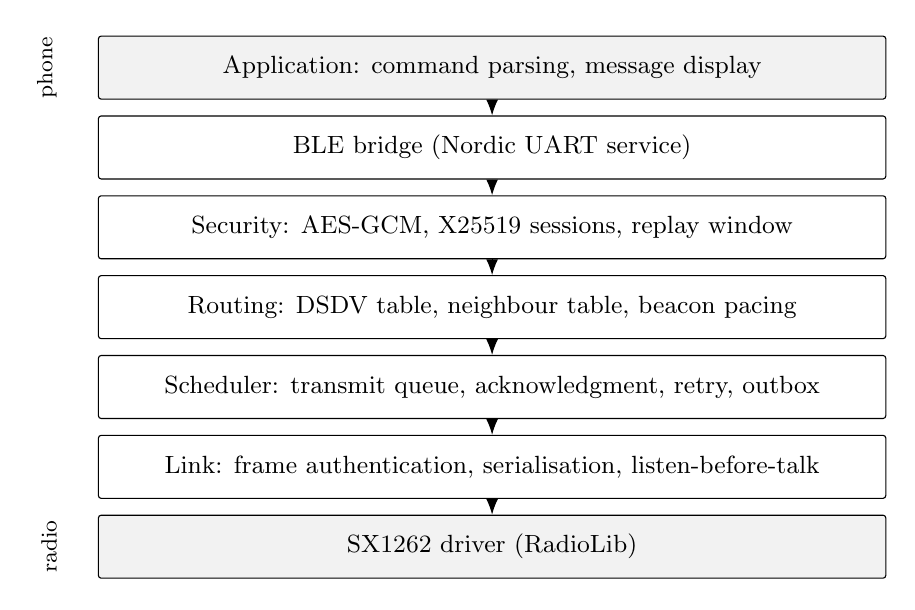
\begin{tikzpicture}[
  font=\small,
  lay/.style={draw, rectangle, minimum width=10cm, minimum height=8mm,
              align=center, rounded corners=1pt},
  arr/.style={-{Latex[length=2mm]}}
]
\node[lay, fill=black!5] (app) {Application: command parsing, message display};
\node[lay, below=2mm of app]  (ble)  {BLE bridge (Nordic UART service)};
\node[lay, below=2mm of ble]  (sec)  {Security: AES-GCM, X25519 sessions, replay window};
\node[lay, below=2mm of sec]  (rt)   {Routing: DSDV table, neighbour table, beacon pacing};
\node[lay, below=2mm of rt]   (sch)  {Scheduler: transmit queue, acknowledgment, retry, outbox};
\node[lay, below=2mm of sch]  (link) {Link: frame authentication, serialisation, listen-before-talk};
\node[lay, below=2mm of link, fill=black!5] (phy) {SX1262 driver (RadioLib)};

\foreach \a/\b in {app/ble, ble/sec, sec/rt, rt/sch, sch/link, link/phy}
  \draw[arr] (\a) -- (\b);

\node[left=4mm of app, rotate=90, anchor=south, font=\footnotesize] {phone};
\node[left=4mm of phy, rotate=90, anchor=south, font=\footnotesize] {radio};
\end{tikzpicture}
\caption{Firmware layering. Each layer corresponds to one source module.}
\label{fig:layers}
\end{figure}

\section{Module decomposition}

\begin{table}[htbp]
\centering
\small
\begin{tabular}{@{}p{4.2cm}p{8.3cm}@{}}
\toprule
Module & Responsibility \\
\midrule
\texttt{config.h} & All tunable constants in one place: radio parameters, table
  sizes, timers, limits. \\
\texttt{lora\_manager.h} & Radio initialisation, transmit and receive, channel
  activity detection. \\
\texttt{packet\_manager.h} & Packet structures, serialisation and parsing with
  length validation. \\
\texttt{security\_manager.h} & AES-GCM, HKDF, frame authentication, replay
  window, sequence persistence. \\
\texttt{crypto\_session.h} & X25519 keypair, peer public keys, per-pair session
  key derivation. \\
\texttt{routing\_manager.h} & Neighbour table, DSDV routing table, node
  directory, beacon interval. \\
\texttt{message\_scheduler.h} & Transmit queue, retry and alternate-route logic,
  store-and-forward outbox. \\
\texttt{communication\_manager.h} & Receive path: frame verification, dispatch by
  type, forwarding decisions. \\
\texttt{message\_receiver.h} & Delivery to the application and duplicate
  suppression at the destination. \\
\texttt{ble\_manager.h} & Bluetooth service, line-oriented protocol to the
  phone. \\
\texttt{metrics.h} & Counters and timing instrumentation. \\
\texttt{LoRaMesh.ino} & Setup, main loop, command interface. \\
\bottomrule
\end{tabular}
\caption{Firmware modules. This satisfies NFR7.}
\label{tab:modules}
\end{table}

\section{Frame types}

Seven types share one channel:

\begin{table}[htbp]
\centering
\small
\begin{tabular}{@{}llp{7.4cm}@{}}
\toprule
Type & Reach & Purpose \\
\midrule
\textsc{data}     & routed    & A user message, or a broadcast alert when the
                                destination is the reserved broadcast address. \\
\textsc{ack}      & one hop   & Confirms that the next hop received a frame. \\
\textsc{hello}    & one hop   & Beacon: neighbour discovery, routing updates,
                                public key, node name, battery state. \\
\textsc{alt}      & one hop   & Tells the sender that this next hop has already
                                seen the packet, so another route should be tried. \\
\textsc{key\_req} & routed    & Requests the public key of a node more than one
                                hop away. \\
\textsc{key\_resp}& routed    & Returns it. \\
\textsc{receipt}  & routed    & Tells the original sender that the destination
                                actually received the message. \\
\bottomrule
\end{tabular}
\caption{Frame types.}
\label{tab:frames}
\end{table}

\section{Packet format}

The \textsc{data} header is the design decision everything else rests on, so it
is worth setting out carefully.

It carries two separate pairs of addresses. The \emph{source} and
\emph{destination} identify the two endpoints and are fixed for the life of the
message. The \emph{previous hop} and \emph{next hop} identify the radio link
currently being used and are rewritten by every relay, along with the
time-to-live, which each relay decrements.

The cipher's authenticated-associated-data input covers the source, destination,
message identifier, sequence number and payload length. It deliberately does not
cover the hop fields or the time-to-live. Figure~\ref{fig:frame} shows which
fields fall where.

\begin{figure}[htbp]
\centering
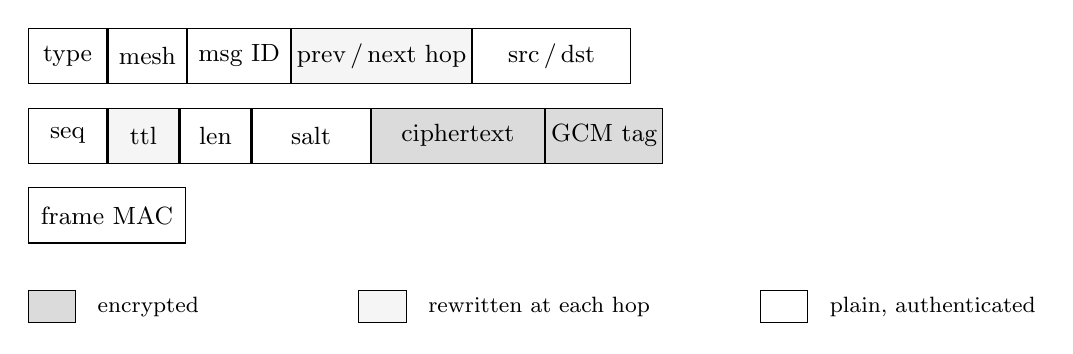
\begin{tikzpicture}[font=\small, node distance=0mm]
\tikzstyle{f}=[draw, minimum height=7mm, align=center, inner sep=2pt]
\tikzstyle{sealed}=[f, fill=black!14]
\tikzstyle{hop}=[f, fill=black!4]
\tikzstyle{open}=[f, fill=white]

\node[open, minimum width=1.0cm] (t)  {type};
\node[open, minimum width=1.0cm, right=of t]  (m)  {mesh};
\node[open, minimum width=1.3cm, right=of m]  (id) {msg ID};
\node[hop,  minimum width=2.0cm, right=of id] (h)  {prev\,/\,next hop};
\node[open, minimum width=2.0cm, right=of h]  (e)  {src\,/\,dst};

\node[open, minimum width=1.0cm, below=3mm of t.south west, anchor=north west] (s) {seq};
\node[hop,  minimum width=0.9cm, right=of s]   (ttl) {ttl};
\node[open, minimum width=0.9cm, right=of ttl] (len) {len};
\node[open, minimum width=1.5cm, right=of len] (salt) {salt};
\node[sealed, minimum width=2.2cm, right=of salt] (ct) {ciphertext};
\node[sealed, minimum width=1.0cm, right=of ct] (tag) {GCM tag};

\node[open, minimum width=2.0cm, below=3mm of s.south west, anchor=north west] (mac) {frame MAC};

% legend: swatch + label, built from ordinary nodes to avoid nesting a
% tikzpicture inside a node
\begin{scope}[font=\footnotesize, shift={($(mac.south west)+(0,-8mm)$)}]
  \node[f, fill=black!14, minimum width=6mm, minimum height=4mm, anchor=west] (l1) at (0,0) {};
  \node[right=1.5mm of l1, anchor=west]  {encrypted};
  \node[f, fill=black!4,  minimum width=6mm, minimum height=4mm, anchor=west] (l2) at (4.2,0) {};
  \node[right=1.5mm of l2, anchor=west]  {rewritten at each hop};
  \node[f, fill=white,    minimum width=6mm, minimum height=4mm, anchor=west] (l3) at (9.3,0) {};
  \node[right=1.5mm of l3, anchor=west]  {plain, authenticated};
\end{scope}
\end{tikzpicture}
\caption{\textsc{data} frame layout. The endpoint addresses are authenticated by
the cipher; the hop addresses are not, because relays must change them. The frame
MAC covers the whole frame and is recomputed at every hop.}
\label{fig:frame}
\end{figure}

This split is what makes end-to-end encryption possible across several hops. An
earlier version of the design used a single pair of address fields for both
purposes, which meant that a relay rewriting the next hop changed a field the
cipher was authenticating, and the destination's tag check failed. Either
encryption or relaying could work, not both. Separating the two pairs resolves
it: relays touch only fields outside the seal, and the destination verifies
exactly the fields that the sender intended and that nobody along the path is
permitted to alter.

A message at the maximum length still fits inside one LoRa transmission, so the
system performs no fragmentation and no reassembly. That was deliberate.
Reassembly across a lossy multi-hop path is a large amount of machinery, and it
is machinery with a long history of being got wrong.

\section{Routing}

\subsection{Sequence numbers and freshness}

Each node owns a sequence number that only it increments, always in steps of two,
so its own advertisements always carry an even value. A route is preferred over
another when its sequence number is higher, or when the sequence numbers are
equal and the hop count is lower.

When a node detects that a link has broken, it advertises that destination with
the sequence number one higher than the last it heard --- an odd number --- and
an infinite metric. Because odd is higher than the even value its neighbours are
holding, the invalidation wins every comparison, and no stale reachable route can
displace it. Only the destination itself can undo it, by issuing the next even
number. This is the mechanism from Perkins and
Bhagwat~\cite{perkins1994dsdv}, and it is what prevents a broken route from
circulating between neighbours with a slowly increasing hop count.

\subsection{Beacons carry the routing table}

Routing updates travel inside the beacon rather than as separate frames. One
beacon therefore carries neighbour discovery, the sending node's routing table,
its public key, its name and its battery voltage. On a channel this slow, a
separate routing protocol would compete with user messages for the same limited
airtime, and there is no reason to pay for two transmissions where one will do.

\subsection{Adaptive beacon interval}

The beacon interval is not fixed. It is computed as the number of nodes the
device knows about, multiplied by the airtime of its own beacon, multiplied by a
constant, and then clamped to a minimum and a maximum.

The reason is arithmetic. If $N$ nodes each beacon every $T$ seconds and each
beacon occupies the channel for $a$ seconds, the permanent load on the shared
channel is $N a / T$. With $T$ fixed, that load grows linearly with $N$; at a
fixed interval, a mesh of twenty nodes spends a large fraction of all available
airtime on beacons alone, and user messages collide with them. Scaling $T$ with
$N$ holds the product roughly constant. The cost is that a large mesh converges
more slowly, which is the correct trade when the alternative is a channel too
congested to carry anything.

Bad news does not wait for the timer. A node that detects a broken link beacons
immediately, so invalidations spread ahead of the scheduled interval. Good news
waits for the next scheduled beacon, which avoids a burst of triggered updates
when a mesh powers on and every node discovers every other at once.

\section{Delivery}

Every hop is acknowledged. An unacknowledged frame is retransmitted a fixed
number of times, after which the sender tries an alternate next hop if the
routing table offers one. If no route works, the message is not discarded: it is
placed in an outbox, still encrypted, and re-sent when a route to the destination
reappears. The outbox is bounded both by a time limit and by an attempt count,
because every attempt costs a transmission and its retries, and retrying
indefinitely against a node that will never return is a waste of shared airtime
rather than a persistence feature.

A hop acknowledgment proves only that one radio heard one frame. It says nothing
about whether the message reached its destination. End-to-end delivery is proved
separately by a receipt that the destination returns, carrying a short
authentication tag computed under the pair's session key. Only the true
destination can compute it. Without that tag any mesh member could fabricate a
delivery confirmation, and the delivery ratio in Chapter~7 would be measuring
nothing.

Broadcast alerts flood rather than route. A node acts on the first copy it sees
and drops the rest, and a time-to-live bounds how far a copy travels, so each
node transmits a given alert at most once.

\section{Security design}

\subsection{Threat model}

Assume an attacker with a LoRa radio within range who can listen to everything,
transmit anything, and record traffic for later. Aras et al.\ demonstrated that
this is not a theoretical position~\cite{aras2017exploring}. Assume also that a
node can be physically captured and its flash read.

The system's security boundary is between mesh members and outsiders. Against an
outsider it provides confidentiality of message content, rejection of forged
routing updates, acknowledgments and receipts, and rejection of replays.

Against a mesh member it provides less, and the report states this plainly rather
than leaving a reader to discover it. A member holds the network key, and can
therefore forge control frames and read broadcasts. What a member still cannot do
is read a one-to-one message that it merely relays, because that requires a
private key it does not have. That single property is what the elliptic-curve
layer exists to provide.

\subsection{Key hierarchy}

\begin{figure}[htbp]
\centering
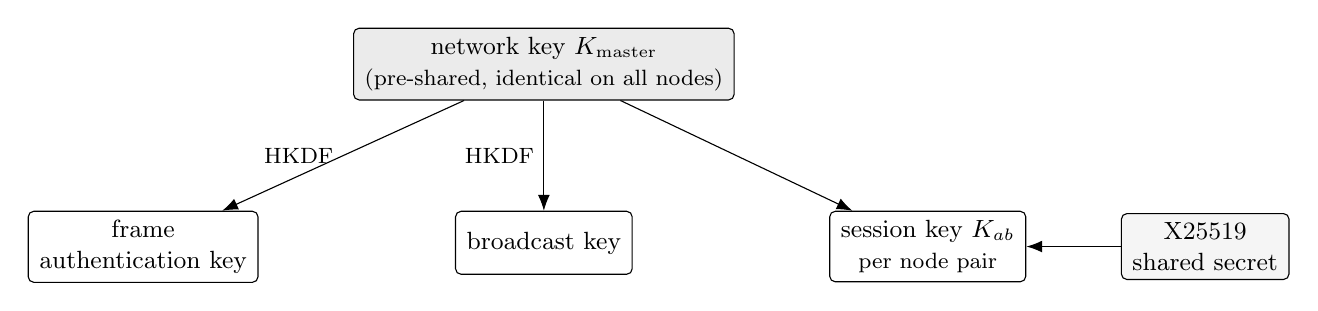
\begin{tikzpicture}[
  font=\small,
  k/.style={draw, rounded corners=2pt, minimum height=8mm, align=center, inner xsep=4pt},
  arr/.style={-{Latex[length=2mm]}}
]
\node[k, fill=black!8] (m) {network key $K_{\text{master}}$\\\footnotesize (pre-shared, identical on all nodes)};

\node[k, below left=14mm and 12mm of m]  (c) {frame\\authentication key};
\node[k, below=14mm of m]                (b) {broadcast key};
\node[k, below right=14mm and 12mm of m] (s) {session key $K_{ab}$\\\footnotesize per node pair};

\node[k, right=12mm of s, fill=black!4] (e) {X25519\\shared secret};

\draw[arr] (m) -- node[left, font=\footnotesize] {HKDF} (c);
\draw[arr] (m) -- node[left, font=\footnotesize] {HKDF} (b);
\draw[arr] (m) -- (s);
\draw[arr] (e) -- (s);
\end{tikzpicture}
\caption{Key derivation. Each key is derived under a distinct context label, so
one cannot be substituted for another. The session key depends on both the
pre-shared key and a per-pair elliptic-curve secret.}
\label{fig:keys}
\end{figure}

Three keys derive from the pre-shared network key using HKDF-SHA256, each under a
different context label so that none can be used in another's
role~\cite{rfc5869}. One authenticates frames. One encrypts broadcasts. The third
is the per-pair session key, and it is not derived from the network key alone.

Each node generates an X25519 keypair the first time it boots and stores the
private half in non-volatile memory. For a pair of nodes $a$ and $b$,

\[
K_{ab} = \mathrm{HKDF}\bigl(\mathit{salt},\;
  X25519(a_{\text{priv}}, b_{\text{pub}}) \,\|\, K_{\text{master}},\;
  \mathit{label} \,\|\, \mathit{lo} \,\|\, \mathit{hi}\bigr)
\]

where $\mathit{lo}$ and $\mathit{hi}$ are the two node identifiers placed in a
fixed order, so that both ends compute the same key without needing to negotiate
which of them is which.

Feeding both the elliptic-curve secret and the pre-shared key into the derivation
means an attacker has to defeat both mechanisms. Recovering the network key from
a captured node is not enough to read one-to-one traffic, and intercepting the
public-key exchange is not enough either. A relay holds $K_{\text{master}}$ like
every other node but holds neither endpoint's private key, so it cannot compute
$K_{ab}$ regardless of how many packets it forwards.

Public keys travel on the beacon, so a session with any direct neighbour costs no
extra exchange. Keys for nodes further away are fetched on demand, when a message
is first addressed to them. An earlier design fetched the public key of every
destination as soon as it appeared in the routing table; the number of exchanges
that requires grows with the square of the mesh size, and in simulation it
dominated the channel while establishing sessions that were mostly never used.

An incoming public key is validated before use. A point of small order yields a
fixed shared secret that the sender can predict without holding any private key,
so such keys are rejected as RFC 7748 requires~\cite{rfc7748}.

\subsection{Message encryption and the nonce}

Payloads are encrypted with AES-128-GCM, which provides confidentiality and
integrity in a single pass and is accelerated in ESP32-S3 hardware. The tag is
checked before any plaintext is released to the application.

GCM has one requirement that cannot be relaxed: a nonce must never repeat under
the same key. The failure is not gradual. Reuse exposes the exclusive-or of the
two plaintexts, and it exposes the authentication subkey, which lets an attacker
forge tags~\cite{dworkin2007gcm}.

The design therefore does not build the nonce from counters. Each message carries
eight bytes drawn from the hardware random number generator at the moment it is
sealed, and the nonce is those bytes followed by the sequence number. Relays
carry the salt unchanged because it is covered by the seal; altering it changes
the nonce, the tag then fails, and the message is discarded. The reason for this
approach, and the defect that made it necessary, are in Section~\ref{sec:nonce}.

\subsection{Replay rejection}

Each node keeps, for every source it has heard from, the highest sequence number
it has accepted and a bitmap of recently seen numbers below it. A message with a
number already marked, or one too old to be in the window, is rejected; one that
arrives out of order but within the window is accepted and marked. Tolerating
out-of-order arrival is necessary rather than generous, because multi-hop routing
reorders messages as a matter of course when a route changes mid-conversation.

The window is consulted only after the authentication tag has verified. The order
matters: if an unauthenticated sequence number were checked first, an attacker
could send forged messages with very high numbers, advance the window, and lock
out the genuine sender without ever needing a key.

Sequence numbers are reserved from non-volatile memory in blocks rather than
written one at a time. A reboot resumes past the whole reserved block, so numbers
are never reused, and flash is not written on every message.

\subsection{Frame authentication}

Every frame carries a truncated HMAC-SHA256 tag computed under the frame
authentication key, and nothing is parsed until it verifies. This is what stops
an outsider injecting beacons. Once routing became table-driven, a forged beacon
would be a serious matter: an attacker could claim a one-hop route to any node
and attract its traffic, which is a routing attack that needs no cryptographic
break at all. Tags are compared without short-circuiting on the first differing
byte, so a failed comparison does not leak how much of a guess was right.

On \textsc{data} frames this tag sits beneath the end-to-end GCM tag and is
recomputed at each hop, because relays legitimately rewrite the hop fields.

\section{Phone interface}

The node exposes a Bluetooth Low Energy service using the Nordic UART profile,
which behaves like a serial port and requires no pairing ceremony. Communication
is a line-oriented text protocol: the phone sends commands, the node sends
messages, status lines and diagnostics.

Bluetooth Classic is not an option. The ESP32-S3 supports only Bluetooth Low
Energy, unlike the original ESP32, so a design assuming a classic serial profile
would not run on this hardware.

The phone application is a web application using the Web Bluetooth API. It is
installable to the home screen and cached, so after one installation it runs with
no network connection of any kind, which matters given where these nodes are
meant to be used. It shows conversations by node name, the list of known nodes
with signal strength and whether a session key has been established, delivery
status per message, and a diagnostics view exposing every firmware command.

Position sharing uses the phone's own receiver rather than a module on the node.
A shared position travels as an ordinary encrypted message with a recognised
prefix, so it is confidential exactly like any other message and requires no
firmware support.

One consequence of the Web Bluetooth choice has to be stated. Web Bluetooth is
unavailable on iOS in every browser, because Apple requires all iOS browsers to
use the same underlying engine; installing a different browser does not change
this. iPhone users need a third-party browser that bridges Bluetooth natively, or
a native iOS application would have to be written.

% =====================================================================
\chapter{Implementation}
% =====================================================================

\section{Toolchain}

The firmware is C++ built with PlatformIO under the Arduino-ESP32 framework. The
radio is driven through RadioLib, which presents the SX1262 and the older SX1276
behind a common interface, so an alternate board can be supported by changing a
compile-time definition. Cryptography uses mbedTLS as shipped with the ESP-IDF,
which supplies hardware-accelerated AES-GCM, SHA-256 and Curve25519 arithmetic.
HKDF is implemented over the available HMAC because the HKDF module is not
enabled in the stock configuration; the implementation was checked against the
test vectors in RFC 5869~\cite{rfc5869}.

The PlatformIO board definition is \texttt{heltec\_wifi\_lora\_32\_V3}, which
matches the hardware directly. Pin assignments are nonetheless taken from the
project's own configuration header rather than from the board definition, so
that the alternate targets can be selected by changing a single macro.

\section{Radio handling}
\label{sec:lbt}

The radio interrupt does one thing: it sets a flag. Reading the frame, and
everything above that, happens in the main loop. Nothing touches SPI from
interrupt context, which avoids a class of intermittent fault that is
unpleasant to diagnose after the fact.

Before transmitting, a node runs channel activity detection using the
transceiver's own hardware, which answers within a few milliseconds. The original
design listened on a fixed window before every frame. That window was long enough
that three hops of it consumed most of the 5\,s latency budget in NFR2 before any
actual radio time was counted. Hardware detection gives the same collision
avoidance at a fraction of the delay, and a short randomised wait before
transmitting handles the case of two nodes deciding to transmit at the same
instant.

\section{Memory and table sizing}

Every table in the system has a fixed size set in the configuration header:
routes, neighbours, known nodes, session keys, replay sources, queued messages,
outbox entries and duplicate history. There is no dynamic allocation in the
message path. On a device with limited RAM and no memory protection, a fixed
ceiling that is reached and reported is better behaviour than an allocation that
succeeds until the day it does not.

The current firmware occupies roughly 19.6\% of available RAM and 33.6\% of flash
on the primary target, and all three build targets compile without warnings.

\section{Instrumentation}

The firmware counts messages sent, first-hop acknowledgments, end-to-end
receipts, retransmissions, frames relayed, duplicates suppressed, and security
events by category. It times encryption and decryption per operation in
microseconds, and accumulates transmit airtime so that duty cycle can be
computed. These counters exist so that Chapter~7 can report measurements rather
than impressions, and they are readable from the phone and from the serial
console.

\section{Problems encountered}

This section records the design problems that came up during implementation and
what was done about them. They are included because the reasoning is part of the
work, and because several of them changed the design rather than just the code.

\subsection{Encryption and relaying were incompatible}

Described in Chapter~4: a single pair of address fields could not serve both the
endpoints and the hops. Relays rewrote a field the cipher authenticated, and the
destination's tag check failed every time. The resolution was to split the
addresses into two independent pairs and to define the authenticated input to
cover only the endpoint pair. Everything else in the security design depends on
that split being right.

\subsection{Nonce reuse after a storage erase}
\label{sec:nonce}

The original nonce was assembled from the sequence number and a message counter.
Both live in non-volatile storage. The broadcast key does not: it is derived from
a network key compiled into the firmware, so it survives a storage erase
unchanged while both counters restart from zero.

The consequence is that the first broadcast sent after erasing storage uses
exactly the nonce of the first broadcast sent before it, under the same key.
That is the one thing GCM does not tolerate. It exposes the exclusive-or of the
two plaintexts and the authentication subkey that lets an attacker forge
tags~\cite{dworkin2007gcm}. Reflashing a node during development triggers it, so
this was not a remote possibility.

The fix removes the dependency on persistent state. Eight bytes from the hardware
random number generator are drawn when the message is sealed and carried in the
frame, and the nonce is those bytes followed by the sequence number. Because the
salt is covered by the authenticated input, a relay cannot alter it without
invalidating the tag, so it needs no protection of its own. A test that
reproduces the original collision and confirms its absence afterwards is part of
the test suite described in Chapter~6.

\subsection{Beacons crowding out messages}

Simulation at twenty nodes showed channel occupancy so high that user messages
had little chance of getting through. The cause was a fixed beacon interval
combined with a beacon that had grown to carry routing information, public keys
and names. The fix was the adaptive interval in Chapter~4: scale the interval
with the number of known nodes so that aggregate control load stays roughly
constant instead of growing with the mesh.

\subsection{Key discovery growing quadratically}

The first key-exchange design fetched a public key for every destination as soon
as it appeared in the routing table. In a mesh of $N$ nodes that is on the order
of $N^2$ exchanges, most of them to set up sessions that are never used, and in
simulation it dominated the channel. Changing to on-demand fetching, triggered by
the first message actually addressed to a node, roughly halved the total frames
at larger sizes.

\subsection{A retry fix that made delivery worse}

The outbox originally freed its slot whenever it re-sent a message, which meant
the attempt counter restarted each time and the cap on attempts never took
effect. The obvious correction was to hold the entry until a receipt confirms
delivery. That correction was right, but the retry interval used with it was long
enough that delivery under node churn fell noticeably in simulation compared with
the earlier, broken behaviour.

The reason turned out to be that the first retry is not like the later ones: when
the first retry goes out there is no earlier copy still travelling through the
mesh for it to collide with, so a long wait before it buys nothing. Making the
first retry interval shorter than the subsequent ones recovered the loss while
keeping the attempt cap working. This is recorded because it is a good
illustration of a fix being correct and still needing measurement: the logic was
right and the constants were wrong, and only the simulation showed it.

\subsection{Injection through the phone protocol}

The protocol between node and phone is line-oriented text. Node names and message
text were being passed into it without filtering, which meant a message
containing a newline followed by text shaped like a status line would be parsed
by the phone as a status line. A user could forge a delivery confirmation for a
message that was never delivered, or make a message appear to come from another
node. Both the node name and the message text are now filtered before they enter
the protocol, and the test suite includes cases for it.

\subsection{Replay window locking out a rebooted peer}

A node that has its storage erased restarts its sequence numbers. Its peers still
hold a replay window with a high water mark, so every message from the returning
node was rejected as a replay, permanently.

The resolution follows from what replay protection is for. It protects within one
key epoch: a message captured under an old key cannot decrypt under a new one, so
once a new session key is agreed with a peer, the old window protects nothing.
The window for that peer is now cleared whenever a new session key is
established, which restores communication with a returning node without weakening
anything.

% =====================================================================
\chapter{Testing Methodology}
% =====================================================================

Testing has three parts, and the report keeps them separate because they prove
different things and it would be misleading to present them as one body of
evidence.

\section{Host-side tests}

The security and protocol algorithms are transcribed into Python and tested on a
desktop, against adversarial inputs rather than only the expected ones. The suite
covers seven areas: packet parsing, AES-GCM, frame authentication, replay
rejection, DSDV route selection, broadcast flooding, and the line protocol
between node and phone. It currently contains 78 tests and all of them pass.

The cases are chosen to try to break the implementation rather than to confirm
it. Parsing is tested against truncation at every possible length, against a
declared payload length that disagrees with the actual frame, and against several
thousand random byte sequences, with the requirement that none of them causes an
exception. Frame authentication is tested against every single-bit alteration of
a frame, each of which must be rejected. Replay rejection is tested at both edges
of the window. Route selection is tested for the absence of count-to-infinity
over repeated exchange rounds. Each defect in Section~5.5 that could be
reproduced has a test that fails against the old behaviour and passes against the
new one, so that a future change cannot quietly reintroduce it.

The limitation of this approach must be stated: these tests exercise a Python
transcription of the algorithms, not the compiled firmware. They can show that
the algorithm is right. They cannot show that the C++ implementing it is right.
HKDF and X25519 are additionally checked against the published test vectors in
RFC 5869 and RFC 7748, which at least anchors those two to an external
reference~\cite{rfc5869,rfc7748}.

\section{Simulation}

A discrete-time simulator models the protocol across a shared channel. It
computes time on air from the standard LoRa equation~\cite{semtech2013toa} and
treats any overlap at a receiver as a lost frame, which is pessimistic, since
real receivers can often recover the stronger of two overlapping signals. It
reimplements routing, key discovery, acknowledgment, flooding and
store-and-forward from the firmware headers, and its constants are checked
against the firmware configuration so that the two cannot drift apart unnoticed.

It does not execute the firmware. It therefore cannot find defects in that code,
and no claim in Chapter~7 about the behaviour of the firmware may rest on it.
What it can do is show how the protocol behaves at sizes larger than five nodes,
which is otherwise unanswerable with the hardware available.

Planned runs: 3, 10 and 20 nodes; a scenario with nodes failing and rejoining;
and a partition in which the field is split into two groups and later rejoined.
Recorded for each: time to converge, end-to-end delivery ratio, latency
distribution, peak occupancy of each table against its configured limit, per-node
duty cycle and collision rate.

\section{Hardware trials}

Five nodes, in three arrangements:

\begin{enumerate}
\item All nodes within direct range of each other, which establishes a baseline
      where routing is not exercised.
\item A line, with nodes placed so that the endpoints are two and then three hops
      apart.
\item A layout offering two disjoint paths between the endpoints, so that an
      intermediate node can be removed without partitioning the mesh.
\end{enumerate}

Measurements come from the instrumentation described in Section~5.4, read over
the phone or the serial console.

Delivery ratio is end-to-end receipts divided by messages sent, measured at the
sender. First-hop acknowledgment ratio is recorded alongside it, because the
difference between the two localises where loss is happening: if hop
acknowledgments are high and receipts are low, the problem is beyond the first
link.

Latency is measured on a single node's own clock, from the moment a message is
queued to the moment it is acknowledged. This avoids needing synchronised clocks
across the mesh, which is not achievable with this hardware, but it means the
figure understates true end-to-end time on a multi-hop path. Chapter~7 must
report it as what it is and not as end-to-end latency.

Planned trials: delivery and latency against hop count; range on a clear
line-of-sight path, against NFR1; behaviour when a relay is switched off during a
conversation and switched back on, including whether held messages are delivered;
broadcast coverage from each origin; time from power-on to a converged routing
table; cryptographic processing time per message, against NFR5; and current draw,
against NFR6.

\section{What has not been tested}

Nothing in this system has run on radio hardware. Specifically unverified: actual
range and received signal strength, channel activity detection under real
contention, interrupt latency, SPI behaviour at speed, the battery measurement
circuit, Bluetooth throughput and reconnection against a real phone, the web
application on a real handset, stack depth under load, and behaviour on brown-out
or watchdog reset.

The audit of this project was carried out by a member of the team who also wrote
the code being audited. That process did find defects, including one introduced
by an earlier fix, which is some evidence that it has value. It is not a
substitute for review by someone who did not write the security layer.

% =====================================================================
\chapter{Results}
% =====================================================================

% =====================================================================
%  PLACEHOLDER — NOTHING HERE YET.
%
%  Hardware trials have not been run. Do not fill this chapter with
%  simulation output written as though it were measurement. If you report
%  simulation figures, put them in their own section and say "simulated"
%  in the text, the table caption AND the figure caption.
%
%  Structure to follow once the data exists:
%    7.1  Simulated behaviour at 3, 10 and 20 nodes
%    7.2  Delivery ratio and latency by hop count (measured)
%    7.3  Range measurements against NFR1
%    7.4  Recovery from node loss and rejoin
%    7.5  Broadcast coverage
%    7.6  Cryptographic cost per message against NFR5
%    7.7  Current draw against NFR6
%    7.8  Requirement-by-requirement outcome table
% =====================================================================

\textit{[Placeholder. Hardware trials described in Chapter~6 have not yet been
carried out. This chapter will present measured results, with simulation results
reported separately and labelled as such.]}

% =====================================================================
\chapter{Conclusion and Future Work}
% =====================================================================

\section{Conclusion}

The project set out to build text messaging over LoRa with no gateway and with
end-to-end confidentiality, and the firmware implements that. Nodes discover each
other, build and maintain routes, relay for each other, and recover when a node
disappears. Messages are encrypted for their destination under a key the two
endpoints agree between themselves, so a relay carries ciphertext it cannot read
even though it holds the network key. Every frame is authenticated at the link
layer, replays are rejected, delivery is confirmed by a receipt the destination
proves cryptographically, and a message for an absent node is held rather than
dropped. A phone acts as the interface over Bluetooth Low Energy.

The design decision that made the rest possible was separating the addresses a
relay rewrites from the addresses the destination authenticates. Without it,
encryption and multi-hop relaying are mutually exclusive, which is why several
published LoRa mesh implementations provide the second and omit the first.

Some conclusions have to wait. Whether the system meets its range, latency and
delivery targets is a question about radios in a field, and that measurement has
not been made. Chapter~7 is reserved for it, and it should be filled only with
numbers taken from the hardware.

Two requirements are known not to be met. Low-power sleep is not implemented,
because a sleeping node neither hears beacons nor relays for others, and the
duty-cycled listening scheme that would resolve that was out of scope. Forward
secrecy is absent: session keys are long-lived, so an attacker who later obtains
a node's private key can decrypt traffic recorded earlier.

\section{Future work}

\textbf{Sleep scheduling.} A coordinated listening schedule would let nodes sleep
between windows without becoming invisible to the mesh, which is what NFR6
requires and what battery life in a real deployment depends on.

\textbf{Forward secrecy.} Rotating session keys on a schedule, or per
conversation, would limit the damage from a key recovered later. The
infrastructure for it exists, since sessions are already established
dynamically.

\textbf{Key revocation.} A captured node's key is valid until every node is
reflashed. A revocation mechanism that does not need a server is a genuinely
difficult problem and would be substantial work on its own.

\textbf{Native iOS application.} Web Bluetooth is unavailable on iOS, which rules
out a large fraction of users. A native application would remove that
restriction.

\textbf{Adaptive radio parameters.} Spreading factor is fixed. Choosing it per
link from measured signal strength would let short links run faster and use less
airtime, leaving more of the channel for the links that need the slow setting.

\textbf{Larger deployment.} Behaviour beyond twenty nodes is untested even in
simulation, and the table sizes in the configuration would need revisiting before
that could be attempted.

% =====================================================================
\bibliographystyle{IEEEtran}
\bibliography{references}
\addcontentsline{toc}{chapter}{References}

\end{document}
